\documentclass[12pt,a4paper]{article}

% ─── Page Layout ───────────────────────────────────────────────────────────────
\usepackage[a4paper, margin=0.8in, headheight=14pt]{geometry}

% ─── Fonts (XeLaTeX) ───────────────────────────────────────────────────────────
\usepackage{fontspec}
\usepackage{unicode-math}
\setmainfont{TeX Gyre Pagella}
\setmonofont[Scale=0.88]{TeX Gyre Cursor}
\setmathfont{Latin Modern Math}

% ─── Packages ──────────────────────────────────────────────────────────────────
\usepackage{xcolor}
\usepackage{colortbl}
\usepackage{titlesec}
\usepackage{enumitem}
\usepackage{tabularx}
\usepackage{booktabs}
\usepackage{array}
\usepackage{amsmath}
\usepackage{tikz}
\usetikzlibrary{shapes.geometric, arrows.meta, positioning, calc, fit, decorations.pathreplacing}
\usepackage{tcolorbox}
\tcbuselibrary{skins, breakable}
\usepackage{hyperref}
\usepackage{fancyhdr}
\usepackage{graphicx}
\usepackage{microtype}
\hyphenpenalty=10000
\exhyphenpenalty=10000
\sloppy
\usepackage{caption}
\usepackage{setspace}
\usepackage{multirow}
\usepackage{tocloft}

% ─── Q&A helper ────────────────────────────────────────────────────────────────
\newcommand{\Q}[1]{\textbf{#1}\par\noindent\ignorespaces}

% ─── Colour Palette ────────────────────────────────────────────────────────────
\definecolor{myred}{RGB}{196,30,58}
\definecolor{mydark}{RGB}{30,30,50}
\definecolor{mygreen}{RGB}{14,120,80}
\definecolor{myteal}{RGB}{0,130,140}
\definecolor{myamber}{RGB}{180,100,0}
\definecolor{mypurple}{RGB}{100,30,160}
\definecolor{mygray}{RGB}{246,247,249}
\definecolor{mgframe}{RGB}{180,185,200}
\definecolor{watermark}{RGB}{145,150,170}
\definecolor{hdrred}{RGB}{250,232,235}
\definecolor{hdrgreen}{RGB}{220,244,233}
\definecolor{hdrteal}{RGB}{220,242,244}
\definecolor{hdramber}{RGB}{253,242,215}
\definecolor{hdrpurple}{RGB}{238,228,255}
\definecolor{hdrgray}{RGB}{238,240,245}
\definecolor{rowalt}{RGB}{250,251,253}

% ─── Section Formatting ────────────────────────────────────────────────────────
\titleformat{\section}
  {\large\bfseries\color{myred}}{\thesection.}{0.5em}{}
  [\vspace{1pt}{\color{myred}\rule{\linewidth}{0.8pt}}]
\titleformat{\subsection}
  {\normalsize\bfseries\color{myteal}}{\thesubsection}{0.5em}{}
\titlespacing*{\section}{0pt}{18pt}{7pt}
\titlespacing*{\subsection}{0pt}{11pt}{4pt}

% ─── Paragraph ─────────────────────────────────────────────────────────────────
\setlength{\parindent}{0pt}
\setlength{\parskip}{4pt}

% ─── TOC Styling ───────────────────────────────────────────────────────────────
\renewcommand{\cfttoctitlefont}{\large\bfseries\color{myred}}
\renewcommand{\cftaftertoctitle}{\par\noindent{\color{myred}\rule{\linewidth}{0.8pt}}}
\setlength{\cftbeforetoctitleskip}{0pt}
\setlength{\cftaftertoctitleskip}{6pt}
\renewcommand{\cftsecfont}{\normalsize\bfseries\color{mydark}}
\renewcommand{\cftsecpagefont}{\normalsize\bfseries\color{mydark}}
\renewcommand{\cftsecleader}{\cftdotfill{\cftdotsep}}
\setlength{\cftbeforesecskip}{7pt}
\renewcommand{\cftsubsecfont}{\small\color{mydark}}
\renewcommand{\cftsubsecpagefont}{\small\color{mydark}}
\setlength{\cftbeforesubsecskip}{3pt}
\setlength{\cftsubsecindent}{1.4em}

% ─── Table helpers ─────────────────────────────────────────────────────────────
\renewcommand{\arraystretch}{1.45}
\setlength{\tabcolsep}{6pt}
\arrayrulecolor{mydark}
\newcolumntype{B}[1]{>{\small\bfseries\raggedright\arraybackslash}m{#1}}
\newcolumntype{Y}{>{\small\raggedright\arraybackslash}X}
\renewcommand{\tabularxcolumn}[1]{m{#1}}

% ─── Header / Footer ───────────────────────────────────────────────────────────
\pagestyle{fancy}
\fancyhf{}
\fancyhead[L]{\small\color{myred}\textbf{PE-EC801A}\;\color{mydark}--- Antennas and Propagation}
\fancyhead[R]{\small\color{myteal}\textbf{Module 3 Notes}}
\fancyfoot[C]{\small\color{mydark}\thepage}
\fancyfoot[R]{\small\color{watermark}\textit{\copyright\ Biraj}}
\renewcommand{\headrulewidth}{0.5pt}
\renewcommand{\footrulewidth}{0.3pt}

% ─── Hyperref ──────────────────────────────────────────────────────────────────
\hypersetup{
  colorlinks=true, linkcolor=myteal, urlcolor=myteal,
  pdfauthor={Biraj Sarkar},
  pdftitle={PE-EC801A --- Module 3 Notes}
}

% ─── tcolorbox styles ──────────────────────────────────────────────────────────
\tcbset{
  tikzbox/.style={
    colback=mygray, colframe=mgframe, boxrule=0.6pt, arc=4pt,
    left=8pt, right=8pt, top=6pt, bottom=6pt,
    colbacktitle=mgframe, coltitle=mydark,
    fonttitle=\small\bfseries
  },
  defbox/.style={
    colback=hdrgreen, colframe=mygreen, boxrule=0.8pt, arc=4pt,
    left=9pt, right=9pt, top=6pt, bottom=6pt,
    colbacktitle=mygreen, coltitle=white,
    fonttitle=\small\bfseries
  },
  formulabox/.style={
    colback=hdrteal, colframe=myteal, boxrule=0.8pt, arc=4pt,
    left=9pt, right=9pt, top=7pt, bottom=7pt,
    colbacktitle=myteal, coltitle=white,
    fonttitle=\small\bfseries
  },
  examplebox/.style={
    colback=hdramber, colframe=myamber, boxrule=0.8pt, arc=4pt,
    left=9pt, right=9pt, top=6pt, bottom=6pt,
    colbacktitle=myamber, coltitle=white,
    fonttitle=\small\bfseries
  },
  masonbox/.style={
    colback=hdrpurple, colframe=mypurple, boxrule=0.8pt, arc=4pt,
    left=9pt, right=9pt, top=6pt, bottom=6pt,
    colbacktitle=mypurple, coltitle=white,
    fonttitle=\small\bfseries
  },
  exambox/.style={
    colback=hdrpurple, colframe=mypurple, boxrule=1pt, arc=5pt,
    left=10pt, right=10pt, top=8pt, bottom=8pt,
    colbacktitle=mypurple, coltitle=white,
    fonttitle=\bfseries,
    breakable, title after break={\textbf{Frequently Asked / Viva Questions (contd.)}}}
}
\tcbset{breakable}

% ─── TikZ styles ───────────────────────────────────────────────────────────────
\tikzset{
  block/.style={rectangle, draw=myteal, fill=hdrteal,
    text width=2.4cm, align=center, minimum height=0.95cm,
    font=\small, rounded corners=3pt, line width=0.7pt},
  redblock/.style={rectangle, draw=myred, fill=hdrred,
    text width=2.4cm, align=center, minimum height=0.95cm,
    font=\small, rounded corners=3pt, line width=0.7pt},
  netnode/.style={rectangle, draw=myteal, fill=hdrteal,
    text width=1.5cm, align=center, minimum height=0.8cm,
    font=\small, rounded corners=3pt, line width=0.7pt},
  sumjunc/.style={circle, draw=myamber, fill=hdramber,
    minimum size=0.62cm, font=\small, line width=0.8pt},
  snode/.style={circle, draw=mypurple, fill=hdrpurple,
    minimum size=0.55cm, font=\footnotesize, line width=0.7pt},
  arrow/.style={-Stealth, thick, color=mydark},
  redarrow/.style={-Stealth, thick, color=myred},
  line/.style={thick, color=mydark}
}

% ═══════════════════════════════════════════════════════════════════════════════
\begin{document}
% ═══════════════════════════════════════════════════════════════════════════════

\begin{center}
  {\LARGE\bfseries\color{myred} PE-EC801A --- Antennas and Propagation}\\[5pt]
  {\normalsize\color{mydark} Semester VIII \quad$\bullet$\quad 3L:0T:0P \quad$\bullet$\quad 3 Credits}\\[3pt]
  {\normalsize\color{myteal}\textbf{Module 3 Exam Notes}}\\[3pt]
  {\small\color{mydark} CGEC \;$|$\; B.Tech ECE (2023--27) \;$|$\; \textit{Biraj Sarkar}}
\end{center}
\vspace{2pt}
\noindent{\color{myred}\rule{\linewidth}{1.5pt}}
\vspace{2pt}

\hypersetup{linkcolor=mydark}
\tableofcontents
\hypersetup{linkcolor=myteal}
\newpage

% ===============================================================================
\section{Huygens' Principle and Field Equivalence}
% ===============================================================================

\begin{tcolorbox}[defbox, title={\textbf{Huygens' Principle}}]
\textbf{Huygens' Principle} states that each point on a primary wavefront behaves as a source of secondary spherical wavelets. These wavelets propagate outward at the speed of the wave in the medium, and the new wavefront at any subsequent time is the envelope of these secondary wavelets.
\end{tcolorbox}

\subsection{Field Equivalence Principle}
In electromagnetics, Schelkunoff's Equivalence Principle allows us to replace actual source currents inside a closed surface $S$ with equivalent electric ($\vec{J}_s$) and magnetic ($\vec{M}_s$) currents on the surface $S$ such that the fields outside $S$ remain unchanged:
\[
\vec{J}_s = \hat{n} \times \vec{H}
\]
\[
\vec{M}_s = -\hat{n} \times \vec{E}
\]
where $\hat{n}$ is the unit outward normal vector to the surface $S$, and $\vec{E}$, $\vec{H}$ are the fields on $S$. This is critical for solving radiation patterns of aperture antennas.

\begin{tcolorbox}[tikzbox, title={Huygens' Wavelet propagation}]
\centering
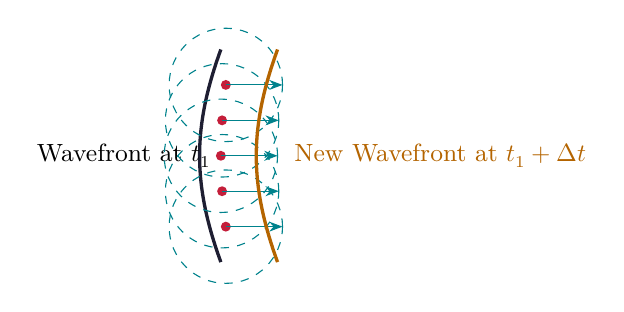
\begin{tikzpicture}[scale=0.9]
  % Original wavefront
  \draw[very thick, color=mydark] (0,-1.5) to[bend left=20] (0,1.5);
  \node[left, font=\small] at (0,0) {Wavefront at $t_1$};

  % Wavelet centers
  \foreach \y in {-1.0, -0.5, 0.0, 0.5, 1.0} {
    \fill[myred] (0.07*\y*\y, \y) circle (0.07);
    \draw[color=myteal, dashed, thin] (0.07*\y*\y, \y) circle (0.8);
    \draw[-Stealth, color=myteal, thin] (0.07*\y*\y, \y) -- +(0.8,0);
  }

  % New wavefront (envelope)
  \draw[very thick, color=myamber] (0.8,-1.5) to[bend left=20] (0.8,1.5);
  \node[right, font=\small\color{myamber}] at (0.9,0) {New Wavefront at $t_1 + \Delta t$};
\end{tikzpicture}
\end{tcolorbox}

% ===============================================================================
\section{Radiation from Apertures}
% ===============================================================================

Aperture antennas (like waveguides, horns, and reflectors) radiate through an opening in their structure. The radiated fields in the far field are proportional to the spatial Fourier transform of the field distribution across the aperture.

\subsection{Rectangular Aperture (Uniform Distribution)}
Consider a rectangular aperture of dimensions $a$ (along $x$) and $b$ (along $y$) in an infinite ground plane. If the aperture field is uniform and $x$-polarized, $\vec{E}_a = \hat{a}_x E_0$, the far-field pattern is:
\[
E(\theta, \phi) \propto \text{sinc}\left( \frac{ka}{2} \sin\theta \cos\phi \right) \text{sinc}\left( \frac{kb}{2} \sin\theta \sin\phi \right)
\]
where $\text{sinc}(x) = \frac{\sin x}{x}$.
\begin{itemize}[leftmargin=*, itemsep=3pt]
  \item \textbf{Maximum Directivity:}
  \[
  D_{max} = \frac{4\pi}{\lambda^2} A_p = \frac{4\pi}{\lambda^2} (ab)
  \]
  \item \textbf{Beamwidth (HPBW):}
  \[
  \text{HPBW}_{E\text{-plane}} \approx 50.6^\circ \frac{\lambda}{b}, \quad \text{HPBW}_{H\text{-plane}} \approx 50.6^\circ \frac{\lambda}{a}
  \]
\end{itemize}

\subsection{Circular Aperture (Uniform Distribution)}
For a circular aperture of radius $a$ with a uniform field, the far-field pattern is described by a Bessel function:
\[
E(\theta) \propto \frac{J_1(ka \sin\theta)}{ka \sin\theta}
\]
where $J_1$ is the first-order Bessel function.
\begin{itemize}[leftmargin=*, itemsep=3pt]
  \item \textbf{Maximum Directivity:}
  \[
  D_{max} = \frac{4\pi}{\lambda^2} A_p = \frac{4\pi}{\lambda^2} (\pi a^2) = \left( \frac{2\pi a}{\lambda} \right)^{\!2}
  \]
  \item \textbf{First Null Angle:} $\theta_{null} \approx 1.22 \frac{\lambda}{2a}$.
  \item \textbf{First Sidelobe Level:} $17.6\,\text{dB}$ below the main beam peak.
\end{itemize}

% ===============================================================================
\section{Babinet's Principle and Slot Antennas}
% ===============================================================================

\subsection{Babinet's Principle}
In optics, Babinet's Principle states that the sum of the diffraction fields behind two complementary screens (where the transparent areas of one screen correspond to the opaque areas of the other) equals the field of the source when no screen is present.

\subsection{Electromagnetic Extension (Booker's Relation)}
H. G. Booker extended Babinet's principle to account for electromagnetic vector properties (polarization and boundary conditions). It relates the input impedance of a slot antenna ($Z_{slot}$) to the impedance of its complementary metal strip dipole ($Z_{dipole}$):

\begin{tcolorbox}[formulabox, title={\textbf{Booker's Impedance Relation}}]
For complementary slot and dipole antennas in free space:
\[
Z_{slot} Z_{dipole} = \frac{\eta_0^2}{4}
\]
where $\eta_0 \approx 377\,\Omega \approx 120\pi$ is the intrinsic impedance of free space.
\end{tcolorbox}

Substituting $\eta_0 \approx 120\pi$:
\[
Z_{slot} Z_{dipole} = \frac{(120\pi)^2}{4} \approx 35476\,\Omega^2
\]
\textbf{Implications:}
\begin{itemize}[leftmargin=*, itemsep=3pt]
  \item Since a resonant thin dipole has $Z_{dipole} \approx 73\,\Omega$, its complementary slot antenna has a resonant input impedance of:
  \[
  Z_{slot} = \frac{35476}{73} \approx 485\,\Omega
  \]
  \item The polarization of the slot antenna is orthogonal to that of the dipole. A vertical slot antenna radiates horizontally polarized waves, whereas a vertical dipole radiates vertically polarized waves.
\end{itemize}

% ===============================================================================
\section{Horn Antennas}
% ===============================================================================

A \textbf{horn antenna} is a flared waveguide that provides a smooth transition from waveguide impedance to free-space impedance, producing high directivity.

\subsection{Types of Horns}
\begin{itemize}[leftmargin=*, itemsep=3pt]
  \item \textbf{E-Plane Sectoral Horn:} Flared only in the direction of the electric field ($E$-field).
  \item \textbf{H-Plane Sectoral Horn:} Flared only in the direction of the magnetic field ($H$-field).
  \item \textbf{Pyramidal Horn:} Flared in both E and H directions. It has a rectangular aperture.
  \item \textbf{Conical Horn:} Circular waveguide flared into a cone.
\end{itemize}

\begin{tcolorbox}[tikzbox, title={Horn Antenna Structures}]
\centering
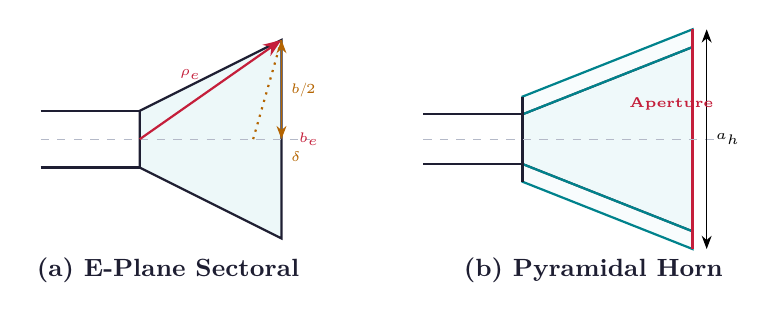
\begin{tikzpicture}[scale=0.9]
  % ── (a) E-Plane Sectoral Horn ──────────────────────────────────────────────
  \begin{scope}[xshift=-4.2cm]
    % Waveguide walls (side view)
    \draw[thick, color=mydark] (-2.0, 0.4) -- (-0.6, 0.4);
    \draw[thick, color=mydark] (-2.0, -0.4) -- (-0.6, -0.4);
    % Flared aperture (E-plane flares vertically)
    \draw[thick, color=mydark, fill=hdrteal, fill opacity=0.5]
      (-0.6, 0.4) -- (1.4, 1.4) -- (1.4, -1.4) -- (-0.6, -0.4) -- cycle;
    % Back wall
    \draw[thick, color=mydark] (-0.6, 0.4) -- (-0.6, -0.4);
    % Center axis
    \draw[dashed, color=mgframe] (-2.0, 0) -- (1.8, 0);
    % Slant length annotation
    \draw[color=myred, -Stealth, thick] (-0.6,0) -- (1.4,1.4) node[midway, above left, font=\tiny] {$\rho_e$};
    % Path difference
    \draw[Stealth-Stealth, thin, color=myamber] (1.4,0) -- (1.4,1.4) node[midway, right, font=\tiny] {$b/2$};
    % Aperture label
    \node[right=3pt, font=\tiny\bfseries\color{myred}] at (1.4, 0) {$b_e$};
    \node[font=\small\bfseries\color{mydark}] at (-0.2,-1.85) {(a) E-Plane Sectoral};
    % Phase error arrows
    \draw[dotted, thick, color=myamber] (1.0,0) -- (1.4, 1.4);
    \node[font=\tiny\color{myamber}] at (1.6,-0.25) {$\delta$};
  \end{scope}

  % ── (b) Pyramidal Horn ─────────────────────────────────────────────────────
  \begin{scope}[xshift=1.4cm]
    % Front face waveguide (top)
    \draw[thick, color=mydark] (-0.8, 0.35) -- (-2.2, 0.35);
    \draw[thick, color=mydark] (-0.8, -0.35) -- (-2.2, -0.35);
    % Left side flap (H-plane)
    \draw[thick, color=mydark] (-0.8, 0.35) -- (-2.2, 0.35);
    % Pyramid outline (top view approximation)
    % Top face
    \draw[thick, color=mydark, fill=hdrteal, fill opacity=0.45]
      (-0.8, 0.35) -- (1.6, 1.3) -- (1.6, -1.3) -- (-0.8, -0.35) -- cycle;
    % H-plane (width) flare shown as offset overlay
    \draw[thick, color=myteal, fill=hdrteal, fill opacity=0.2]
      (-0.8, 0.35) -- (-0.8, 0.6) -- (1.6, 1.55) -- (1.6, 1.3) -- cycle;
    \draw[thick, color=myteal, fill=hdrteal, fill opacity=0.2]
      (-0.8, -0.35) -- (-0.8, -0.6) -- (1.6, -1.55) -- (1.6, -1.3) -- cycle;
    % Aperture lip
    \draw[very thick, color=myred] (1.6, -1.55) -- (1.6, 1.55);
    % Back wall
    \draw[thick, color=mydark] (-0.8, 0.6) -- (-0.8, -0.6);
    \draw[thick, color=mydark] (-2.2, 0.35) -- (-0.8, 0.35);
    \draw[thick, color=mydark] (-2.2, -0.35) -- (-0.8, -0.35);
    % Axis
    \draw[dashed, color=mgframe] (-2.2, 0) -- (2.0, 0);
    % Dimension labels
    \draw[Stealth-Stealth, thin] (1.8, -1.55) -- (1.8, 1.55) node[midway, right, font=\tiny] {$a_h$};
    \node[font=\small\bfseries\color{mydark}] at (0.2,-1.85) {(b) Pyramidal Horn};
    \node[font=\tiny\bfseries\color{myred}] at (1.3,0.5) {Aperture};
  \end{scope}
\end{tikzpicture}
\end{tcolorbox}

\subsection{Design Concepts and Path Length Difference}
Flaring the waveguide causes a phase variation across the horn's aperture because waves traveling to the outer edge of the horn travel a longer path length ($\rho$) than waves traveling along the center axis. 
The maximum path difference $\delta$ is:
\[
\delta = \rho \left( 1 - \cos\frac{\theta}{2} \right) \approx \frac{b^2}{8\rho}
\]
where $b$ is the aperture height and $\rho$ is the horn length.
To prevent destructive interference, $\delta$ must be kept within limit:
\begin{itemize}[leftmargin=*, itemsep=2pt]
  \item For $E$-plane horn: $\delta_{max} < \lambda / 4 \implies b^2 < 2 \lambda \rho_e$.
  \item For $H$-plane horn: $\delta_{max} < 3\lambda / 8 \implies a^2 < 3 \lambda \rho_h$.
\end{itemize}

% ===============================================================================
\section{Reflector Antennas}
% ===============================================================================

Reflector antennas use a metallic surface to redirect and focus electromagnetic waves from a primary source (feed) into a highly directive beam.

\subsection{Prime-Focus Parabolic Reflector}
A paraboloidal reflector is a surface of revolution formed by rotating a parabola about its axis. A primary feed (e.g., dipole or small horn) is placed at the focal point $F$.

\begin{tcolorbox}[tikzbox, title={Parabolic Reflector Configurations}]
\centering
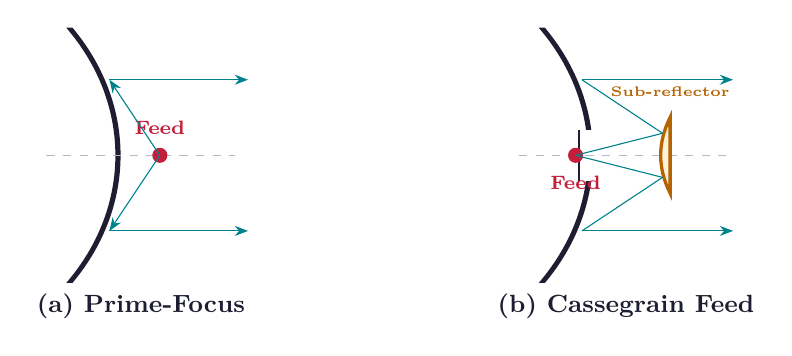
\begin{tikzpicture}[scale=0.8]
  % Prime Focus Reflector
  \begin{scope}[xshift=-4cm]
    % Draw parabola
    \draw[very thick, color=mydark, fill=hdrgray] 
      (-0.8, 2.0) .. controls (0.2, 0.8) and (0.2, -0.8) .. (-0.8, -2.0) -- 
      (-0.83, -2.0) .. controls (0.17, -0.8) and (0.17, 0.8) .. (-0.83, 2.0) -- cycle;
      
    % Axis
    \draw[dashed, color=mgframe] (-1.2, 0) -- (1.8, 0);
    
    % Focal point feed
    \fill[myred] (0.6, 0) circle (0.12) node[above=4pt, font=\scriptsize\bfseries] {Feed};
    
    % Ray tracing
    \draw[color=myteal, -Stealth] (0.6,0) -- (-0.2, 1.2);
    \draw[color=myteal, -Stealth] (-0.2, 1.2) -- (2.0, 1.2);
    \draw[color=myteal, -Stealth] (0.6,0) -- (-0.2, -1.2);
    \draw[color=myteal, -Stealth] (-0.2, -1.2) -- (2.0, -1.2);
    
    \node[font=\small\bfseries\color{mydark}] at (0.3,-2.4) {(a) Prime-Focus};
  \end{scope}

  % Cassegrain Reflector
  \begin{scope}[xshift=3.5cm]
    % Draw main parabola
    \draw[very thick, color=mydark, fill=hdrgray] 
      (-0.8, 2.0) .. controls (0.2, 0.8) and (0.2, -0.8) .. (-0.8, -2.0) -- 
      (-0.83, -2.0) .. controls (0.17, -0.8) and (0.17, 0.8) .. (-0.83, 2.0) -- cycle;
      
    % Hole in main reflector
    \fill[white] (-0.35, -0.4) rectangle (0.05, 0.4);
    \draw[thick, color=mydark] (-0.25, 0.4) -- (-0.25, -0.4);
    
    % Axis
    \draw[dashed, color=mgframe] (-1.2, 0) -- (2.2, 0);
    
    % Sub-reflector (hyperbolic)
    \draw[very thick, color=myamber, fill=hdramber] 
      (1.2, 0.6) .. controls (1.0, 0.2) and (1.0, -0.2) .. (1.2, -0.6) -- cycle;
    \node[above=4pt, font=\tiny\bfseries\color{myamber}] at (1.2, 0.6) {Sub-reflector};
      
    % Actual feed at vertex
    \fill[myred] (-0.3, 0) circle (0.12) node[below=4pt, font=\scriptsize\bfseries] {Feed};
    
    % Rays
    \draw[color=myteal] (-0.3,0) -- (1.08, 0.35);
    \draw[color=myteal] (1.08, 0.35) -- (-0.2, 1.2);
    \draw[color=myteal, -Stealth] (-0.2, 1.2) -- (2.2, 1.2);
    
    \draw[color=myteal] (-0.3,0) -- (1.08, -0.35);
    \draw[color=myteal] (1.08, -0.35) -- (-0.2, -1.2);
    \draw[color=myteal, -Stealth] (-0.2, -1.2) -- (2.2, -1.2);
    
    \node[font=\small\bfseries\color{mydark}] at (0.5,-2.4) {(b) Cassegrain Feed};
  \end{scope}
\end{tikzpicture}
\end{tcolorbox}

\textbf{Characteristics:}
\begin{itemize}[leftmargin=*, itemsep=3pt]
  \item Converts a spherical wavefront radiating from the feed into a highly directive plane wavefront.
  \item All path lengths from the feed to the reflector and out to the aperture plane are identical: $r + r\cos\theta = 2f$.
  \item The $f/D$ ratio (focal length to diameter) is a critical design parameter that determines the curvature of the dish and feed antenna illumination requirements.
\end{itemize}

\subsection{Cassegrain Antenna (Dual-Reflector)}
A \textbf{Cassegrain antenna} uses a primary parabolic main reflector and a secondary hyperbolic sub-reflector.
\begin{itemize}[leftmargin=*, itemsep=3pt]
  \item \textbf{Setup:} The primary feed horn is placed at a convenient location, usually at the vertex of the main reflector. The sub-reflector is positioned between the feed and the main focus.
  \item \textbf{Ray Path:} Spherical waves from the feed are reflected by the hyperbolic sub-reflector, directing them toward the main parabolic reflector as if they originated from the paraboloid's focus. The main reflector then reflects them as a collimated plane wave.
\end{itemize}

\par\noindent
\textbf{Cassegrain Advantages:}\par\noindent
{\renewcommand{\arraystretch}{1.45}%
\begin{tabularx}{\linewidth}{|B{3.5cm}|Y|}
\hline
\textbf{Feature} & \textbf{Cassegrain Advantage} \\
\hline
Feed Line Loss & Feed is at the vertex; eliminates long, lossy feed lines to the focus. \\
\hline
Noise Temperature & Feed looks up at the cold sky (via sub-reflector) rather than down at the warm, noisy earth, reducing receiver noise. \\
\hline
Structural Support & Heavy feed equipment (amplifiers, cryogenics) is mounted behind the dish, rather than being suspended at the focus. \\
\hline
\end{tabularx}}

% ===============================================================================
% MANDATORY QUICK REVISION PAGE
% ===============================================================================
\newpage
\begin{center}
  {\large\bfseries\color{myred} Quick Revision --- Module 3}\\[3pt]
  {\small\color{mydark} Aperture and Reflector Antennas $|$ PE-EC801A}
\end{center}
\noindent{\color{myred}\rule{\linewidth}{1.2pt}}
\vspace{4pt}

\begin{tcolorbox}[formulabox, title={\textbf{Key Formulas and Metrics at a Glance}}]
\renewcommand{\arraystretch}{1.35}
\begin{tabularx}{\linewidth}{B{5.2cm} X}
Aperture Max Directivity & $D_{max} = \frac{4\pi}{\lambda^2} A_p$ \quad (uniform distribution) \\[4pt]
Circular Apertity Null & $\theta_{null} \approx 1.22 \frac{\lambda}{2a}$ \\[4pt]
Booker's Relation & $Z_{slot} Z_{dipole} = \frac{\eta_0^2}{4} \approx 35476\,\Omega^2$ \\[4pt]
Resonant Slot Impedance & $Z_{slot} \approx 485\,\Omega$ \quad (complementary to $73\,\Omega$ dipole) \\[4pt]
Horn Flare Limit (E-plane) & $b^2 < 2\lambda\rho_e$ \quad (limits phase error to $< \pi/2$) \\[4pt]
Horn Flare Limit (H-plane) & $a^2 < 3\lambda\rho_h$ \quad (limits phase error to $< 3\pi/4$) \\[4pt]
Parabola Equation & $y^2 = 4fx$ \quad ($f$ = focal length) \\
\end{tabularx}
\end{tcolorbox}

\begin{tcolorbox}[defbox, title={\textbf{One-Line Definitions}}]
\begin{itemize}[leftmargin=*, itemsep=2pt, topsep=0pt]
  \item \textbf{Equivalence Principle:} A principle allowing actual source fields inside a closed boundary to be replaced by equivalent surface currents.
  \item \textbf{Aperture Efficiency:} The ratio of the effective aperture of an antenna to its physical aperture area.
  \item \textbf{Complementary Screens:} Two screens where the open areas of one correspond to the closed areas of the other.
  \item \textbf{Optimum Horn:} A horn antenna whose dimensions are chosen to achieve maximum gain for a fixed flare length.
  \item \textbf{Spillover Loss:} Power radiated by the feed antenna that misses the reflector dish and is lost.
  \item \textbf{Cassegrain Antenna:} A dual-reflector system using a parabolic main reflector and a hyperbolic sub-reflector.
\end{itemize}
\end{tcolorbox}

\begin{tcolorbox}[exambox, title={\textbf{Frequently Asked / Viva Questions}}]
\begin{enumerate}[topsep=0pt, label=\textbf{Q\arabic*.}, itemsep=5pt]
  \item \Q{State Babinet's principle and its electromagnetic extension (Booker's relation).}
    Babinet's principle states that the sum of the fields behind complementary screens equals the source field without screens. Booker's relation extends this to EM fields, showing that for a slot antenna and its complementary dipole, $Z_{slot} Z_{dipole} = \frac{\eta_0^2}{4}$.
  \item \Q{Why does a slot antenna have a high input impedance compared to a dipole?}
    By Booker's relation, $Z_{slot} Z_{dipole} \approx 35476$. Because a resonant dipole has $Z_{dipole} \approx 73\,\Omega$, its complementary slot antenna has a high impedance: $Z_{slot} = \frac{35476}{73} \approx 485\,\Omega$.
  \item \Q{Compare the polarization of a vertical slot antenna and a vertical dipole.}
    They are orthogonal. A vertical dipole radiates vertically polarized waves, whereas a vertical slot antenna radiates horizontally polarized waves (because the electric field lines span horizontally across the vertical slot).
  \item \Q{Why are horn antennas flared? What happens if the flare angle is too large?}
    Flaring provides a gradual impedance match from the waveguide to free space, reducing reflections. If the flare angle is too large, the path difference between central and edge rays becomes large, causing phase errors that degrade gain and increase sidelobes.
  \item \Q{What are the advantages of a Cassegrain reflector over a prime-focus parabolic reflector?}
    \begin{itemize}[leftmargin=*, itemsep=1pt, topsep=2pt]
      \item Lower transmission line loss because the feed is located at the vertex.
      \item Lower noise temperature since the feed points upward at the cold sky.
      \item Easy installation and maintenance of heavy feed and receiver electronics.
    \end{itemize}
  \item \Q{Explain the trade-off involved in the $f/D$ ratio of a parabolic reflector.}
    A small $f/D$ (deep dish) reduces spillover but requires a wide-angle feed, which is hard to design with uniform phase. A large $f/D$ (flat dish) simplifies feed design but increases spillover loss and requires a longer, heavier feed structure.
  \item \Q{State the field equivalence principle and its use in aperture antennas.}
    It allows replacing the actual sources inside a closed surface with equivalent electric and magnetic currents on the surface. It simplifies analyzing slot, horn, or aperture antennas by integrating fields across the aperture rather than calculating currents on complex conductors.
\end{enumerate}
\end{tcolorbox}

\begin{tcolorbox}[tikzbox, title={Comparison of Aperture Antenna Types}]
\centering
\renewcommand{\arraystretch}{1.55}
{\renewcommand{\arraystretch}{1.55}%
\begin{tabularx}{\linewidth}{|B{3.0cm}|Y|Y|Y|}
\hline
\multicolumn{1}{|>{\centering\arraybackslash}m{3.0cm}|}{\textbf{Parameter}} &
\multicolumn{1}{>{\centering\arraybackslash}Y|}{\textbf{Slot Antenna}} &
\multicolumn{1}{>{\centering\arraybackslash}Y|}{\textbf{Horn Antenna}} &
\multicolumn{1}{>{\centering\arraybackslash}Y|}{\textbf{Parabolic Reflector}} \\
\hline
Directivity / Gain & Low to Medium & Medium ($10$–$25\,\text{dB}$) & Very High ($30$–$50\,\text{dB}$) \\
\hline
Bandwidth & Narrow (resonant) & Wide (waveguide band) & Extremely Wide \\
\hline
Impedance & High ($\approx 485\,\Omega$) & Matched to waveguide & Matches feed antenna \\
\hline
Typical Applications & Aircraft, radar arrays & Feed for reflectors, gain standards & Satellite TV, radar, radio astronomy \\
\hline
\end{tabularx}}
\end{tcolorbox}

\end{document}
